%!TEX ROOT=formularioFisica.tex

\section{Magnetismo}\label{sec:magnetismo}
Il magnetismo si occupa del campo magnetico e dei suoi effetti. Ogni magnete genera un
campo magnetico ($\vec{B}$). La sua direzione è sempre dal polo NORD a quello SUD. Ogni magnete ha
sempre due poli e anche se lo si divide si otterranno magneti bipolari.\\ 
L'unità di misura di $\vec{B}$ è il \emph{Tesla} ($T = \frac{N}{Am}$)\\
Si noti che $\mu = \mu_0\mu_r$ e \hyperref[tab:mu0]{$\mu_0$}: $4\pi\cdot10^{-7}\,\text{N/A}^2$.\\
Per gli esercizi si vada a pagina~\pageref{ex:magnetismo}.

\subsection{Forza in un campo magnetico}
Un filo in cui scorre una corrente, immerso in un campo magnetico $B$, è sottoposto ad una forza
pari a
\begin{equation*}	
  \vec{F} = l\cdot(\vec{i}\times\vec{B})
\end{equation*}
Questo è un \hyperref[subsec:vettori:prodottoVettoriale]{prodotto vettoriale}. Si usi la regola
della mano.\\
$l$ rappresenta la lunghezza del cavo che attraversa il campo magnetico\\
$\vec{i}$: è la corrente che attraversa il cavo. Il verso può essere positivo o
negativo in base al sistema di riferimento scelto.

\subsection{Legge di Biot-Savart}
La legge di Biot-Savant mostra la stretta relazione tra campo elettrico e magnetico. Definisce un 
campo magnetico generato da un filo rettilineo percorso da una corrente.\\
La direzione è la tangente alla linea di campo generata dal filo, il verso è antiorario se la
corrente esce, orario altrimenti. Un modo per ricordarselo più facilmente è il seguente: si prenda la
mano destra e si usi il pollice per indicare il verso e la direzione della corrente. Si chiudano poi
a pugno le altre dita. Il verso delle dita chiuse, è quello del campo magnetico.
\begin{equation*}
  B = \frac{\mu}{2\pi}\frac{i}{d}
\end{equation*}
$i$: corrente\\
$d$: distanza dal filo\\ [\baselineskip]

In genere negli esercizi si trova disegnato o un cerchio con un punto o uno con una croce che
vengono usati per indicare il verso del filo o del campo, come i seguenti

\begin{center}
  \begin{tikzpicture}
    \tikzset{cross/.style={cross out, draw=black, minimum size=2*(#1-\pgflinewidth),
      inner sep=0pt, outer sep=0pt},
      %default radius will be 1pt. 
      cross/.default={1pt}
    }
    \draw (-1,0) circle (0.3);
    \filldraw (-1,0) circle (0.04);
    \draw (1,0) circle (0.3);
    \draw (1,0) node[cross=3pt]{};
    \node[text width=1.5cm] at (-1,-0.7){Uscente nel foglio};
    \node[text width=1.5cm] at (1,-0.7){Entrante dal foglio};
  \end{tikzpicture}
\end{center}

\subsection{Legge di Ampére}
La legge di Ampére descrive la forza che intercorre tra due fili paralleli attraversati da una
corrente.
\begin{equation*}
  F = \frac{\mu}{2\pi}\frac{i_1i_2}{d}l
\end{equation*}
$i$: corrente\\
$d$: distanza tra i due fili\\
$l$: lunghezza del filo\\ [\baselineskip]
La formula calcola il modulo del vettore. La forza è attrattiva se i versi delle correnti sono 
uguali, repulsiva altrimenti.

\subsection{Solenoidi}
I solenoidi (anche detti bobine) sono degli strumenti che, attraversati da corrente, generano un
campo magnetico uniforme al loro interno mentre all'esterno è $0$. Essi sono composti da spire,
disposte in questo modo
\begin{center} % https://tex.stackexchange.com/questions/129860/helix-on-a-cylinder
  \tdplotsetmaincoords{70}{15}
  \begin{tikzpicture}[tdplot_main_coords, rotate=90, scale=0.5]

    % --- Independent parameters ---
    \def\h{15}                          % cylinder height
    \pgfmathtruncatemacro\tA{299}      % A angle
    \def\zA{1}                         % A applicate
    \pgfmathtruncatemacro\tB{110}      % B angle
    \def\zB{5}                         % B applicate
    \pgfmathtruncatemacro\n{5}         % number of additional turns
    \pgfmathtruncatemacro\NbPt{500}    % number of dots for drawing the helix portion
    \def\rhelixdots{0.05}              % radius of dots forming helix
    \def\rAB{0.05}                     % radius of A and B dots

    % lower circle
    %\draw[black,very thin] (1,0,0) 
    %\foreach \t in {2,3,...,360}
    %{
    %	--({cos(\t)},{sin(\t)},0)
    %}
    %--cycle;

    % upper circle
    %\draw[black,very thin] (1,0,\h) 
    %\foreach \t in {2,4,...,360}
    %{
    %	--({cos(\t)},{sin(\t)},\h)
    %}
    %--cycle;

    % --- Draw helix ---
    \pgfmathsetmacro\tone{\tA}
    \pgfmathsetmacro\tlast{\tB+\n*360}
    \pgfmathsetmacro\ttwo{\tone+(\tlast-\tone)/(\NbPt-1)}
    \pgfmathsetmacro\p{360*(\zB-\zA)/(\tB-\tA+360*\n)}
    \foreach \t in {\tone,\ttwo,...,\tlast}{%
      \fill[black!80] ({cos(\t)},{sin(\t)},{\p*(\t-\tA)/360+\zA}) circle[radius=\rhelixdots];
    }

    % --- Draw A and B ---
    %\fill[blue] ({cos(\tA)},{sin(\tA)},\zA) circle [radius=\rAB]node[right]{$A$};
    %\fill[blue] ({cos(\tB)},{sin(\tB)},\zB) circle [radius=\rAB]node[left]{$B$};
  \end{tikzpicture}
\end{center}
\begin{equation*}
  B = \mu \frac{n}{l}i
\end{equation*}
$n$: numero di spire\\
$l$: lunghezza del solenoide\\
$i$: corrente

\subsection{Energia di un campo magnetico}
In modo analogo al campo elettrico, si può definire un'energia e una densità magnetici. Per fare 
ciò analizziamo un circuito RL in serie. Per Kirchhoff
\begin{equation*}
  \mathcal{E} + \mathcal{E}_{ind} = Ri
\end{equation*}
Dove $\mathcal{E}_{ind}$ è la forza elettromotrice indotta dal solenoide. Sostituendo
\begin{equation*}
  \mathcal{E} -L\der{i}{t} = Ri
\end{equation*}
Moltiplicando ambo i membri per $i\dif t$ per ottenere un'energia
\begin{equation*}
  \mathcal{E} = L\frac{\dif i}{\cancel{\dif t}}i\cancel{\dif t}+Ri^2\dif t
\end{equation*}
Il termine $Ri^2\dif t$ è semplicemente l'effetto Joule. Invece il termine $Li\dif i$ è proprio
l'energia del campo magnetico generato dal solenoide. Quindi dato che a noi serve un valore
complessivo, non istantaneo, integriamo
\begin{equation*}
  U_B = \int_0^i Li\dif i = \left.\frac{Li^2}{2}\right|_0^i = \frac{1}{2}Li^2
  \end{equation*}
  La densità magnetica invece si ricava
  \begin{equation*}
    u_B = \frac{U_B}{Sl} = \frac{1}{2\mu_0}B^2
  \end{equation*}

  \subsection{Motore elettrico}
  Nonostante il nome possa far credere che funzioni solo attraverso l'elettricità, il motore elettrico 
  svolge la sua funzione grazie ad una coesione di elettricità e magnetismo. Il disegno seguente 
  cercherà di chiarire le idee.
  \begin{center}
    \begin{tikzpicture}
      % Magnets
      \coordinate (N1) at (0,1);
      \coordinate (N2) at (0,-1);
      \coordinate (S1) at (3,1);
      \coordinate (S2) at (3,-1);
      % Plate
      \coordinate (P1) at (1,0.5);
      \coordinate (P2) at (2,-0.5);

      % Magnets
      \draw[thick] (-0.5,1) -- (N1) -- (N2) -- (-0.5,-1);
      \draw[thick] (3.5,1) -- (S1) -- (S2) -- (3.5,-1);
      % Plate
      \draw[thick] (P1) -- (P2);

      % Magnetic lines
      \foreach \a in {0.8,0,-0.8}{
        \draw[gray, very thin, -stealth] (0.2, \a) -- ++(2.6,0);
      }

      \draw[-stealth] (P1) -- ++(0,0.7);
      \draw[-stealth] (P2) -- ++(0,-0.7);

      % Annotations
      \node at (-0.5,0){$N$};
      \node at (3.5,0){$S$};
      \node at (1.7,0.3){$P$};
      \node at (0.5,-1.2){$\vec{B}$};
      \node at ($(P1)+(0,0.9)$){$\vec{F}$};
      \node at ($(P2)+(0,-0.9)$){$\vec{F}$};
    \end{tikzpicture}
  \end{center}
  Come funziona? Innanzitutto abbiamo un campo magnetico $N-S$ e una spira rettangolare $P$ attraverso 
  la quale passa corrente (solitamente è caratterizzata da un vasto numero di strati). Si fa passare 
  corrente all'interno di questa spira in modo che una forza si generi. Questa forza metterà in 
  rotazione la spira. Quando si raggiunge la situazione in cui il momento è $0$ (ovvero quando è 
  perpendicolare al campo) la corrente viene invertita così che la piastra continui il giro. Questa 
  forza motrice è quella che si genera e verrà poi usata.\\
  Per capire meglio il movimento si guardi il disegno qua sotto
  \begin{center}
    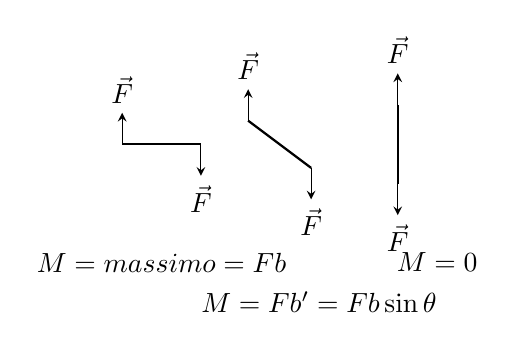
\begin{tikzpicture}
      \coordinate (P1) at (0,0);
      \coordinate (P2) at (1,0);

      \coordinate (P3) at (1.6,0.3);
      \coordinate (P4) at (2.4,-0.3);

      \coordinate (P5) at (3.5,0.5);
      \coordinate (P6) at (3.5,-0.5);

      \draw[thick] (P1) -- (P2);
      \draw[thick] (P3) -- (P4);
      \draw[thick] (P5) -- (P6);

      \draw[-stealth] (P1) -- ++(0,0.4)
        node[pos=1,above]{$\vec{F}$};
      \draw[-stealth] (P2) -- ++(0,-0.4)
        node[pos=1,below]{$\vec{F}$};

      \draw[-stealth] (P3) -- ++(0,0.4)
        node[pos=1,above]{$\vec{F}$};
      \draw[-stealth] (P4) -- ++(0,-0.4)
        node[pos=1,below]{$\vec{F}$};

      \draw[-stealth] (P5) -- ++(0,0.4)
        node[pos=1,above]{$\vec{F}$};
      \draw[-stealth] (P6) -- ++(0,-0.4)
        node[pos=1,below]{$\vec{F}$};

      \node at (0.5,-1.5){$M =\text{ massimo} = Fb$};
      \node at (2.5,-2){$M=Fb'=Fb\sin\theta$};
      \node at (4,-1.5){$M=0$};
    \end{tikzpicture}
  \end{center}

  \subsection{Forza di Lorenz}
  La forza di Lorenz è la forza che una carica in moto risente all'interno di un campo magnetico.
  \begin{equation*}
    \vec{F} = q\vec{v}\times\vec{B}
  \end{equation*}

  Si presti attenzione al verso di questa forza. Se la carica è \emph{positiva} si usi la solita
  regola della mano, altrimenti si inverta semplicemente il verso.\\[\baselineskip]	
  Una particolarità è che una carica che entra in un campo magnetico viene deviata dal suo percorso.
  Il moto che ne deriva è \emph{elicoidale}. Ovviamente questo nel caso più generale, il disegno
  di seguito aiuterà a capire in che modo l'elettrone viene spostato

  \begin{center} % https://tex.stackexchange.com/questions/129860/helix-on-a-cylinder
    \tdplotsetmaincoords{70}{15}
    \begin{tikzpicture}[tdplot_main_coords]

      % --- Independent parameters ---
      \def\h{3}                          % cylinder height
      \pgfmathtruncatemacro\tA{350}      % A angle
      \def\zA{1}                         % A applicate
      \pgfmathtruncatemacro\tB{150}      % B angle
      \def\zB{2}                         % B applicate
      \pgfmathtruncatemacro\n{3}         % number of additional turns
      \pgfmathtruncatemacro\NbPt{100}    % number of dots for drawing the helix portion
      \def\rhelixdots{0.05}              % radius of dots forming helix
      \def\rAB{0.05}                     % radius of A and B dots

      % lower circle
      \draw[black,very thin] (1,0,0) 
        \foreach \t in {2,3,...,360}
        {
          --({cos(\t)},{sin(\t)},0)
        }
        --cycle;

      % upper circle
      \draw[black,very thin] (1,0,\h) 
        \foreach \t in {2,4,...,360}
        {
          --({cos(\t)},{sin(\t)},\h)
        }
        --cycle;

      % --- Draw helix ---
      \pgfmathsetmacro\tone{\tA}
      \pgfmathsetmacro\tlast{\tB+\n*360}
      \pgfmathsetmacro\ttwo{\tone+(\tlast-\tone)/(\NbPt-1)}
      \pgfmathsetmacro\p{360*(\zB-\zA)/(\tB-\tA+360*\n)}
      \foreach \t in {\tone,\ttwo,...,\tlast}{%
        \fill[red!80] ({cos(\t)},{sin(\t)},{\p*(\t-\tA)/360+\zA}) circle[radius=\rhelixdots];
      }

      % --- Draw A and B ---
      \fill[blue] ({cos(\tA)},{sin(\tA)},\zA) circle [radius=\rAB]node[left]{$A$};
      \fill[blue] ({cos(\tB)},{sin(\tB)},\zB) circle [radius=\rAB]node[left]{$B$};
      \draw[thick,-stealth] ({cos(\tA)},{sin(\tA)},\zA) -- ++(0.3,0,0.2)
        node[pos=0.5,below right]{$v_x$};
      \draw[thick,-stealth] ({cos(\tA)},{sin(\tA)},\zA) -- ++(0,0,0.4)
        node[pos=0.5,above right]{$v_y$};
    \end{tikzpicture}
  \end{center}
  Questa è una rappresentazione del moto di una carica all'interno del campo magnetico. Queste formule
  permettono di trovare il \emph{raggio}, \emph{periodo} e il \emph{passo} dell'elica. Nelle
  seguenti formule, si utilizzeranno le due componenti distinte della velocità.
  \begin{alignat*}{2}
    \frac{mv^2_x}{r}&= qv_xB  &\qquad  T &= \frac{2\pi\cdot m}{q\cdot B}\\
    \Delta S &= v_y\cdot T & r&=\frac{mv_x}{qB}
  \end{alignat*}

  \subsection{Selettore di velocità}
  Il selettore di velocità è un particolare dispositivo che permette di "selezionare" alcune cariche che
  vanno solo ad una determinata velocità attraverso una fessura. Il loro utilizzo è molto ampio, 
  specialmente in dispositivi come televisioni a tubo catodico.\\
  Il loro funzionamento si basa su due campi $\vec{E}$ e $\vec{B}$ uniformi incrociati fra di loro.\\
  Sulla carica deve agire una forza $\vec{F}$ pari a
  \begin{equation*}
    \vec{F} = q\vec{E} + q\vec{v}\times\vec{B}
  \end{equation*}
  Una carica passa nel selettore se e solo se la sua velocità è pari a
  \begin{equation*}
    v = \frac{E}{B}
  \end{equation*}

  \subsection{Flusso}
  Il flusso ($\Phi$) di un campo magnetico $\vec{B}$ è pari a 
  \begin{equation*}
    \Phi_S(\vec{B}) = \sum^n_{i=1} \vec{B}\cdot\Delta\vec{S}_i
  \end{equation*}
  Si noti però che il flusso di qualsiasi superficie che insista sulla stessa linea chiusa, avrà
  sempre lo stesso valore.\\
  Il flusso di un solenoide, si trova moltiplicando il numero di spire per il flusso generato da una
  spira.

  \subsection{Legge di Faraday-Neuman-Lenz}\label{subsec:mag:fnl}
  La legge descrive un fenomeno scoperto da Faraday per caso. Un circuito, immerso in un campo
  magnetico, al variare di questo genera una corrente indotta. Più precisamente, al variare
  del flusso del campo magnetico, viene generata una corrente indotta.\\
  Faraday, Neuman e Lenz assieme arrivarono alla formulazione della seguente formula
  \begin{equation*}
    \mathcal{E} = -\frac{\Delta\Phi(\vec{B})}{\Delta t}
  \end{equation*}
  se considerata una media
  \begin{equation*}
    \mathcal{E} = -\frac{\dif\Phi(\vec{B})}{\dif t}
  \end{equation*}
  se considerata istantanea.\\
  In queste formule $\mathcal{E}$ è la forza elettromotrice indotta (dato che con una corrente
  generata, possiamo immaginare ci sia una forza elettromotrice che la genera), $\Phi$ è il flusso
  e $t$ il tempo.\\
  Si noti anche che modificando la formula della forza elettromotrice possiamo dire che
  \begin{equation*}
    \mathcal{E} = vBl
  \end{equation*}
  dove $v$ è la velocità di spostamento del conduttore/circuito in questione, $B$ il campo magnetico
  e $l$ la lunghezza del conduttore.
  \begin{center}
    \begin{tikzpicture}
      \tikzset{cross/.style={cross out, draw=black, minimum size=2*(#1-\pgflinewidth),
        inner sep=0pt, outer sep=0pt},
        %default radius will be 1pt. 
        cross/.default={1pt}
      }
      \foreach \x in {0,0.5,1,...,3}{
        \foreach \y in {0.5,0,-0.5}{
          \draw[thin,lightgray] (\x,\y) circle (0.1);
          \draw (\x,\y) node[thin, lightgray, cross=2pt]{};
        }
      }
      \filldraw[gray] (0.15,0.3) -- ++(0.2,0) -- ++(0,-0.6) -- ++(-0.2,0) -- cycle;
      \draw[-stealth] (0.2,0) -- ++(1,0)
        node[pos=0.5, below]{$\vec{v}$}; 
      \draw[|<->|] (-0.3,0.3) -- ++(0,-0.6)
        node[pos=0.5,left]{$l$};
      \draw[draw=black!60,draw opacity=0.5,line width=2mm] (-1,0.4) -- ++(4,0) -- ++(0,-0.8) -- ++(-4,0);
    \end{tikzpicture}
  \end{center}
  Per fare muovere questa asta di velocità costante, c'è una forza che si contrappone alla forza
  tirante che è pari a
  \begin{equation*}
    \vec{F} = l\vec{i}\times\vec{B}
  \end{equation*}

  \subsection{Circuitazione}
  La circuitazione ($C$) di un campo magnetico $\vec{B}$ è molto simile alla circuitazione
  di un campo elettrico
  \begin{equation*}
    C_\Gamma(\vec{B}) = \sum^{n}_{i=1}\vec{B}_i\cdot\Delta l_i
  \end{equation*}
  $\Delta l$: spostamento

  \subsubsection{Teorema di Ampére}
  Il teorema di Ampére dice che
  \begin{equation*}
    C_\Gamma(\vec{B}) = \mu_0 \sum\limits^{n}_{i=1} i_c
  \end{equation*}
  dove $i_c$ è una corrente concatenata. Una corrente $i$ si definisce concatenata con una linea
  chiusa $\Gamma$ se attraversa una superficie che ha come linea chiusa $\Gamma$.

  \begin{center}
    \begin{tikzpicture}
      [
      decoration={
        markings,
      mark=at position 0.5 with {\arrow{stealth}}}
      ]
      \draw (0,0) ellipse (2 and 0.5);
      \draw[postaction={decorate}] (-0.5,1) -- ++(0,-2)
        node[pos=0.5,left]{$5$A};
      \draw[postaction={decorate}] (0.5,-1) -- ++(0,2)
        node[pos=0.5,right]{$3$A};
    \end{tikzpicture}
  \end{center}

  Preso per esempio il disegno qui sopra, la circuitazione sarebbe
  \begin{equation*}
    C_\Gamma(\vec{B}) = \mu_0(5-3) = 2\mu_0
  \end{equation*}

